\documentclass{standalone}
\usepackage{tikz}
\usepackage{ctex,siunitx}
\setCJKmainfont{Noto Serif CJK SC}
\usepackage{tkz-euclide}
\usepackage{amsmath}
\usetikzlibrary{patterns, calc}
\usetikzlibrary {decorations.pathmorphing, decorations.pathreplacing, decorations.shapes,}
\begin{document}
\small
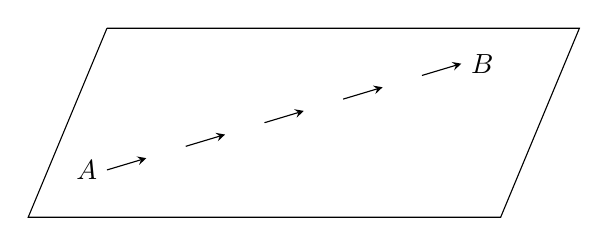
\begin{tikzpicture}[>=stealth,yscale=.6]
  % \useasboundingbox(-4.7,-1.1)rectangle(4.7,2.3);
  \draw(1,4)--(7,4)--(6,0)--(0,0)--(1,4);
  \draw[->](1,1)node[left]{$A$}--(1.5,1.25);
  \draw[->](2,1.5)--(2.5,1.75);
  \draw[->](3,2)--(3.5,2.25);
  \draw[->](4,2.5)--(4.5,2.75);
  \draw[->](5,3)--(5.5,3.25)node[right]{$B$};
\end{tikzpicture}
\end{document}